\section{Semaine 8 : 27/03/2023 - 31/03/2023}
\graphicspath{{semaines/semaine_8/images/}}

\begin{abstract}
	L'idée principale de la semaine et de tester de rehausser la solution. Deux méthodes ont été proposées : rehausser par une constante $m$ (proposée par Emmanuel) ou rehausser par la level-set initial $\phi$ (proposée par Michel).
	
	J'ai également essayé de faire des boxplots pour comparer FEM standard, $\phi$-FEM, FNO et FNO+Corr (pour différents nombres d'époques).
\end{abstract}

\subsection{Rehaussement}

On considère toujours le problème initial

$$\left\{\begin{aligned}
	&-\Delta u=f \quad &&\Omega \\
	&u=0 \quad &&\Gamma
\end{aligned}\right.$$

On prend encore la solution analytique trigonométrique suivante :
$$u_{ex}(x,y) = \frac{1}{\sin\left(k_1\frac{\pi}{2}\right)}\times\sin\left(k_1\frac{\pi}{2}\left(\frac{4}{\sqrt{2}}\right)^2\left((x-0.5)^2+(y-0.5)^2\right)\right)\times\cos\left(\frac{\pi}{2}\left(\frac{4}{\sqrt{2}}\right)^2\left((x-0.5)^2+(y-0.5)^2\right)\right)$$ 

avec $k_1 \sim \mathcal{U}([0.1,1])$.

\subsubsection*{Par une constante}

On considère la solution rehaussée par $m$ :
$$\tilde{\phi}=u+m$$

avec $m$ une constante.

Voici la solution pour $k_1=0.5$ et $m=1$ (à gauche la solution $u$, à droite la solution rehaussée $\tilde{\phi}$) :

\begin{minipage}{\linewidth}
	\centering
	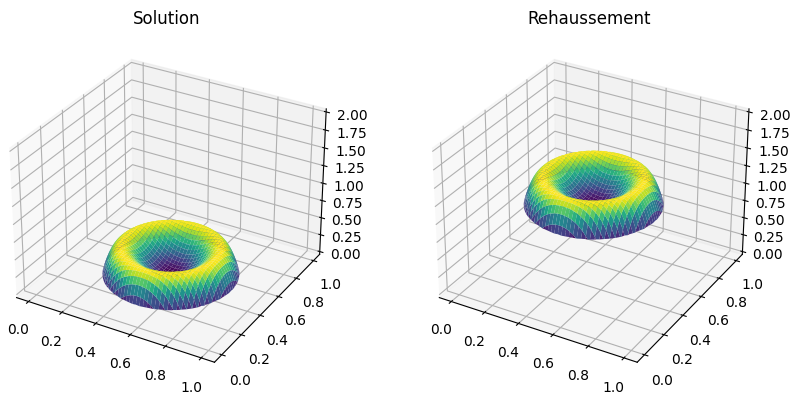
\includegraphics[width=0.5\linewidth]{rehaussement_cste.png}
\end{minipage}

On réécrit alors le problème par

$$\left\{\begin{aligned}
	&-\Delta (\tilde{\phi}-m)=f \quad &&\Omega \\
	&\tilde{\phi}=m \quad &&\Gamma
\end{aligned}\right.$$

Donc

$$\left\{\begin{aligned}
	&-\Delta \tilde{\phi}=f \quad &&\Omega \\
	&\tilde{\phi}=m \quad &&\Gamma
\end{aligned}\right.$$

On veut appliquer la correction, on pose alors $\tilde{u}=\tilde{\phi}C$
avec $\tilde{\phi}$ la level-set.

On a 

$$\left\{\begin{aligned}
	&-\Delta \tilde{u}=f \quad &&\Omega \\
	&\tilde{u}=m \quad &&\Gamma
\end{aligned}\right.$$

On se ramène alors à la correction du problème initial en posant
$$u_c = \tilde{\phi}C-m$$

On prend nb\_data=10. On cherche à comparer la moyenne des erreurs PhiFEM sur les nb\_data données avec la Correction pour différents degré d'intepolation de la levelset et avec la Correction par rehaussement pour différents degré d'interpolation et différents $m$. Voici les résultats obtenus :

\begin{minipage}{\linewidth}
	\centering
	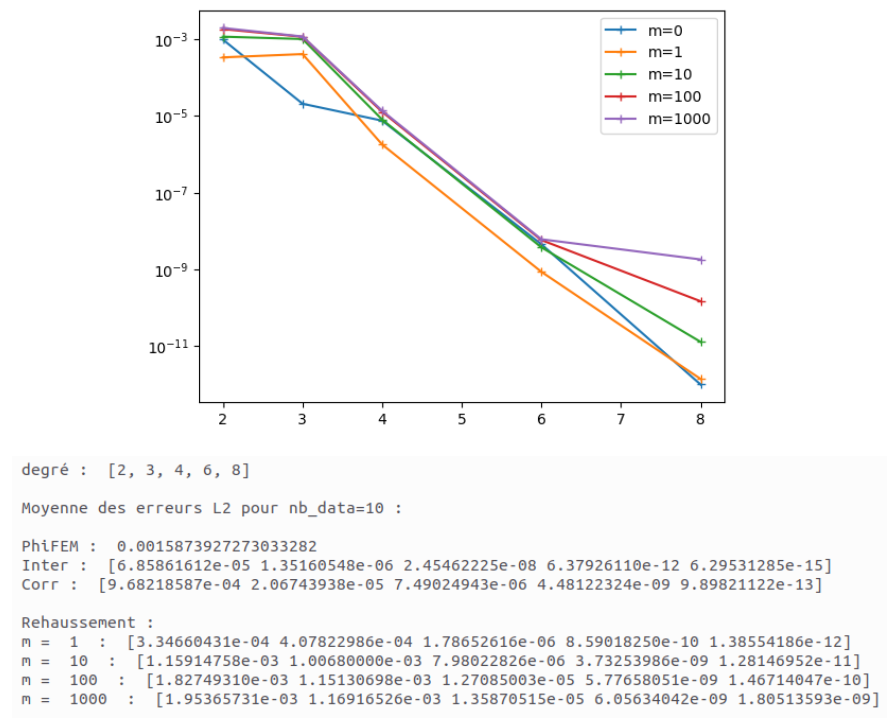
\includegraphics[width=0.8\linewidth]{resultats_cste.png}
\end{minipage}

Et les facteurs obtenus :

\begin{minipage}{\linewidth}
	\centering
	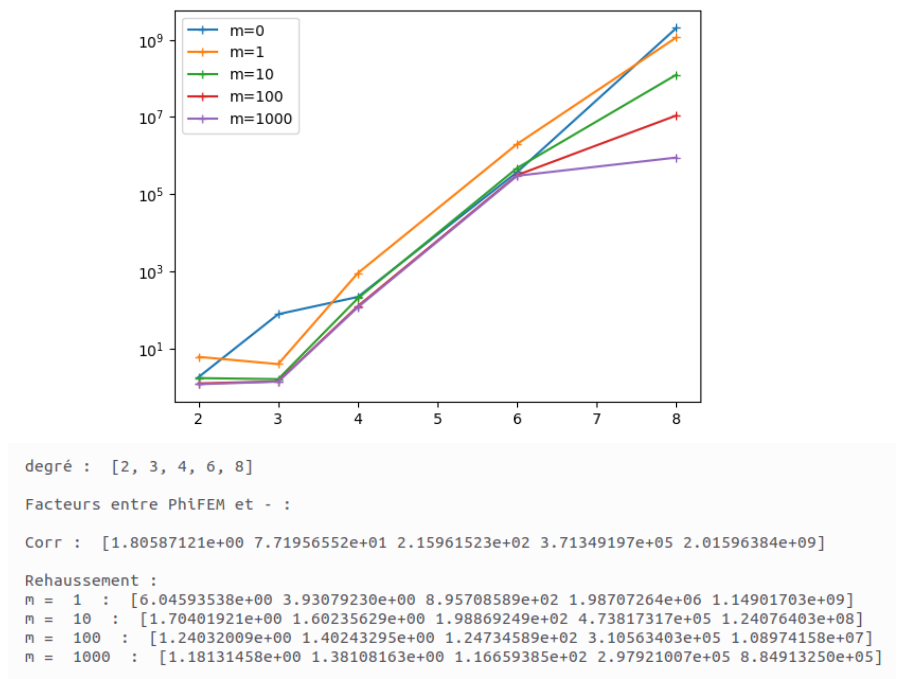
\includegraphics[width=0.8\linewidth]{facteurs_cste.png}
\end{minipage}

\newpage
\subsubsection*{Par la level-set $\phi$}

On considère la solution rehaussée par une constante multipliée par $\phi$ :
$$\tilde{\phi}=u-\alpha\phi$$

avec $\alpha$ une constante positive.

Voici la solution pour $k_1=0.5$ et $\alpha=2$ (à gauche la solution $u$, à droite la solution rehaussée $\tilde{\phi}$) :

\begin{minipage}{\linewidth}
	\centering
	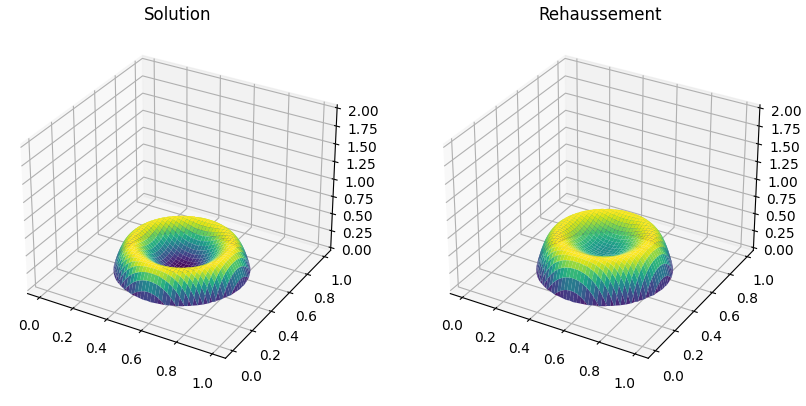
\includegraphics[width=0.5\linewidth]{rehaussement_phi.png}
\end{minipage}

On réécrit alors le problème par

$$\left\{\begin{aligned}
	&-\Delta (\tilde{\phi}+\alpha\phi)=f \quad &&\Omega \\
	&\tilde{\phi}=0 \quad &&\Gamma
\end{aligned}\right.$$

Donc

$$\left\{\begin{aligned}
	&-\Delta \tilde{\phi}=\tilde{f} \quad &&\Omega \\
	&\tilde{\phi}=0 \quad &&\Gamma
\end{aligned}\right.$$

avec $\tilde{f}=f+\alpha\Delta\phi$.

On veut appliquer la correction, on pose alors $\tilde{u}=\tilde{\phi}C$
avec $\tilde{\phi}$ la level-set.

On a 

$$\left\{\begin{aligned}
	&-\Delta \tilde{u}=\tilde{f} \quad &&\Omega \\
	&\tilde{u}=0 \quad &&\Gamma
\end{aligned}\right.$$

On se ramène alors à la correction du problème initial en posant
$$u_c = \tilde{\phi}C+\alpha\phi$$

Voici les résultats obtenus :

\begin{minipage}{\linewidth}
	\centering
	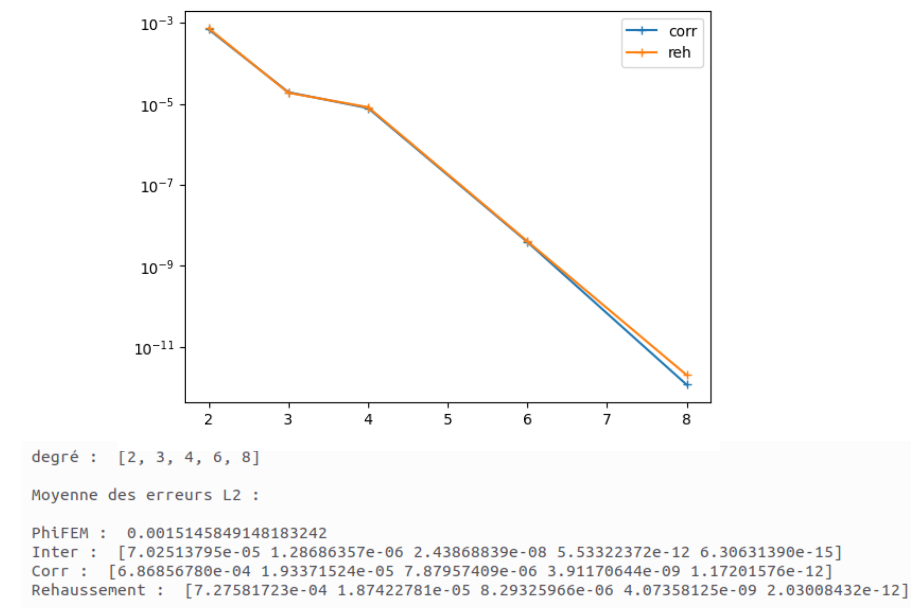
\includegraphics[width=0.7\linewidth]{resultats_phi.png}
\end{minipage}

\subsection{Résultats avec le FNO}

On considère cette fois-ci $f$ gaussienne :
$$f(x,y) = \exp\left(-\frac{(x-\mu_0)^2 + (y-\mu_1)^2}{2\sigma^2}\right)\,, $$ 
avec $\sigma \sim \mathcal{U}([0.1,0.6])$ et $\mu_0, \mu_1 \sim \mathcal{U}([0.5-\sqrt{2}/4, 0.5+\sqrt{2}/4])$ à condition que $\phi(\mu_0, \mu_1) < -0.05$. \\

Dans un premier temps, on considère la solution de référence $u_{ref}$ comme étant une solution sur-raffinée $\mathbb{P}^1$ obtenue par les EF standard (avec $h_{ref}\approx 0.006$ car $h_{ref}<<h_{FNO}$). 

On cherche à afficher des boxplots (boite à moustache) sur les erreurs en norme $L^2$ pour FEM standard, PhiFEM, le FNO et le FNO corrigé pour différents nombres d'époques. On prendra un nouvel échantillon test avec nb\_data=100. 

On va donc comparer
$$||u_{ref}-u_{FEM}||_{L^2,rel}, \quad ||u_{ref}-u_{\phi-FEM}||_{L^2,rel}, \quad ||u_{ref}-u_{FNO}||_{L^2,rel}, \quad ||u_{ref}-Cu_{FNO}||_{L^2,rel}$$

où $u_{FEM}$ est la solution $\mathbb{P}^1$ obtenue par la méthode des éléments finis standard avec une taille de maillage comparable à celle utilisée pour le FNO, $u_{\phi-FEM}$ est la solution $\mathbb{P}^1$ obtenue par $\phi$-FEM, $u_{FNO}$ est la solution $\mathbb{P}^2$ obtenue par le FNO et $C$ est la correction $\mathbb{P}^1$ obtenue en prenant comme level-set $u_{FNO}$.

Voici les résultats obtenus :

\begin{minipage}{\linewidth}
	\centering
	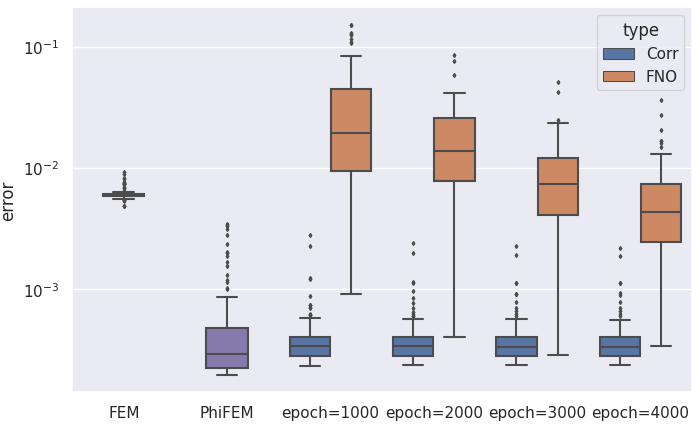
\includegraphics[width=0.7\linewidth]{boxplots.png}
\end{minipage}

\conclusion{Les résultats pour le rehaussement n'ont pas l'air bon : il faudra en parler la semaine prochaine avec Emmanuel et Michel.
	
Pour la partie avec le FNO, la semaine prochaine il faudrait comparer les temps d'exécution entre PhiFEM et FNO+Corr (ratio temps/erreur ou erreur/temps).}